\documentclass[a4paper, twocolumn, 11pt, twoside]{article}

\usepackage{linguamatica}
\usepackage{expex}

\usepackage[brazil]{babel} % Configura o idioma para português do Brasil
\usepackage{linguex}

\usepackage[T1]{fontenc} % To handle special characters
\usepackage[utf8]{inputenc} % To handle UTF-8 encoded characters
\usepackage{amssymb} % For symbols like ? in glosses

\usepackage[x11names]{xcolor}   % For color with explicit color model
\usepackage{graphicx} % For handling images (optional)
\usepackage{fancyhdr} % For custom headers/footers (optional)

%% Please use UTF8 in your document

%% Set the bibliography style.
%% Styles provided for Spanish (Castilian), Catalan and Portuguese.
%% Other languages will be created on a required basis.

\usepackage{linguamatica}
\usepackage{expex}

\bibliographystyle{sp_por}   % This for Portuguese
% \bibliographystyle{sp_esp} % This for Castilian
% \bibliographystyle{sp_cat} % This for Catalan


%% You can leave this unchanged. It will be updated by the editors when your paper gets published.
\submitted{15 de \OCT{} 2024}
\accepted{3 de \DEC{} 2024}


%% Add your title in the main language used in the article
\title{Desafios na Tradução da Informação Espacial do EN-PT-br}

%% Currenty the title in English is also mandatory
\titleEN{Challenges in Translating Spatial Information from EN-PT-br}


%% Add authors here. Three lines for each author.
%% First line with author name, second with the affiliation and third with e-mail
%% In cases where a second line is needed for the affiliation, use the command \nl to separate them. 
\author{
  Rafael Fernandes
  \instituto{Universidade de São Paulo}
  \email{rafael.macario@usp.br} 
  \and 
  Rodrigo Souza
 \instituto{Universidade de São Paulo}
  \email{rodrigo.aparecido.souza@usp.br}
  \and
  Marcos Lopes
  \instituto{Universidade de São Paulo}
  \email{marcoslopes@usp.br}
  \and
%%  Paulo Santos
%%  \instituto{Flinders University}
%%  \email{paulo.santos@flinder.edu.au}
%%%%  \and
%%  Thomas Finbow
%%  \instituto{Universidade de São Paulo}
%%  \email{thomas.finbow@usp.br}
}


\begin{document}
\maketitle

%% Add the abstract in the main language for the article. If possible, doesn't add any citations here.
\begin{resumo}
  A Tradução Automática Neural (TAN), atualmente a abordagem mais utilizada, ainda enfrentam desafios ao lidar com a tradução do conhecimento espacial. Neste estudo, utilizamos o Raciocínio Espacial Qualitativo (REQ) para representar informações espaciais em traduções automáticas do inglês para o português. Traduzimos $145$ frases dos corpora CAM e COCA, utilizando Google Translate e DeepL, e identificamos as causas das traduções não naturais. Com o uso do REQ, mapeamos logicamente as diferenças de significado. Nossos resultados indicam que, apesar de um bom desempenho no geral, a TAN apresenta dificuldades com significados espaciais específicos, resultando em $10,6\%$ de erros semânticos e $12,0\%$ de erros de projeção sintática. Este trabalho explora os desafios práticos e teóricos da tradução automática.
\end{resumo}

%% Add keywords in the article main language, in lowercase
\palavraschave{Tradução Automática Neural; Tradução Automática Inglês-Português; Raciocínio Espacial Qualitativo; Google Translate; DeepL.}


%% Add the abstract in English
\begin{abstract}
\end{abstract}

%% add the keywords in English
\keywords{Open-source LLMs, Neural Machine Translation, Spatial Semantics, Polysemy, Language Typology}


\section{Introdução}
A Tradução Automática Neural (TAN) tornou-se o paradigma dominante na área de Tradução Automática, tanto em estudos acadêmicos quanto em aplicações práticas~\citep{dabre2020survey}~\citep{vaswani2017attention, yang2020survey}. Esse avanço se deve, em grande parte, à capacidade aprimorada dos modelos de aprendizado profundo de captar dependências longas nas frases.

No entanto, apesar dos avanços, alguns tradutores automáticos ainda enfrentam desafios ao lidar com as nuances da linguagem espacial, como a polissemia das preposições e a projeção idiossincrática da maneira de movimento em inglês diretamente para verbos em português~\citep{}. Um exemplo disso pode ser visto no Exemplo (1), retirado do Cambridge Online Dictionary (CAM), onde a tradução do inglês (EN) para o português (PT) foi realizada com o Google Translate (GT) e o DeepL (DL).

\footnotesize
\ex. He swam \emph{across} the river. (CAM)\label{ex:across2}
\ag. ?~Ele nadou do outro lado do rio. (GT) \\  
3SG.M swam from-the other side of-the river\\ 
\bg. Ele atravessou o rio a nado. (DL) \\ 
3SG.M crossed the river by swimming\\
\par
\normalsize

A tradução do Exemplo~\ref{ex:across2} feita pelo modelo GT, embora gramaticalmente correta, erra ao não capturar a expressão mais natural em PT para a sentença em EN. O DL, por outro lado, acerta em cheio.

A razão por trás dessa tradução errada está na polissemiada preposição across, que pode significar tanto uma localização oposta fixa ao ponto de referência quanto movimento de um lado de um espaço para o outro. Neste caso em particular, o significado pretendido é claramente o último. Para ilustrar isso, vamos considerar as Figuras 1 e 2.

\begin{figure}[ht]
  \centering
  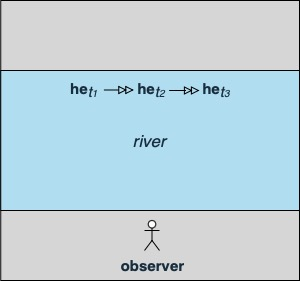
\includegraphics[width=0.3\textwidth]{aa-a-2.jpg}
  \caption{Diagrama semântico de (1)-a.}\label{fig:across-1a}
\end{figure}

\begin{figure}[ht]
  \centering
  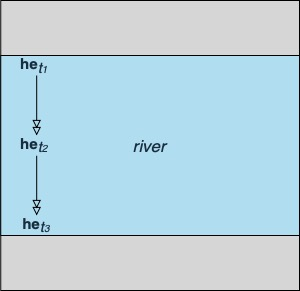
\includegraphics[width=0.3\textwidth]{bb-b-2.jpg}
  \caption{Diagrama semântico de (1)-b.}\label{fig:across-1b}
\end{figure}


A Figura~\ref{fig:across-1a}, representando a saída GT, indica movimento dentro de um local específico (uma margem oposta do rio). No entanto, a Figura 2, representando a saída DL, transmite o significado de cruzar de uma margem do rio para a outra, capturando assim a natureza dinâmica implícita na frase original EN. 

Com isso em mente, este artigo explora a tradução automática de frases em EN que envolvem informações espaciais (topologia ou movimento) para PT, utilizando GT e DL. Nosso objetivo é duplo: primeiro, baseados nos trabalhos de Spranger et al. (2016), Freksa e Kreutzmann (2016) e Randell et al. (1992), formalizamos amostras de frases nas línguas de origem e destino. Em seguida, categorizamos as traduções para identificar erros comuns cometidos por ferramentas de TAN. Em vez de focar no processo de TAN em si, discutiremos os significados espaciais que essas ferramentas têm dificuldade em capturar, iluminando práticas e direções teóricas para pesquisa em linguagem espacial e TA. Nossos resultados mostram que, apesar do bom desempenho geral, os motores de TA ainda cometem erros sistemáticos em algumas categorias ao traduzir textos de EN para PT.


\subsection{Desafios na Tradução da Espacialidade}

A formatação ao longo do documento é a normal em documentos \LaTeX, sem grandes alterações. No entanto,
algumas sugestões:
\begin{itemize}
\item Para dar \emph{ênfase} use sempre que possível o comando \verb.\emph.;
\item Para citar poderá usar o comando \verb.\citep. que cria referências entre
  parêntesis~\citep{latex}. Para citar um \citet{autor}, use o comando \verb.\citet.;
\item Citações seguidas devem reaproveitar o comando de citação. Caso necessite de indicar a página
  a que se refere a citação, use \citep[p.~40]{latex}.
\item Ao criar entradas bibliográficas assegure-se da correção do seu
  conteúdo. Não abrevie nomes de autores. Não coloque os nomes dos
  editores de livros de atas. Não se esqueça dos números das páginas
  do documento.
\item Sempre que usar endereços web e outros tipos de URI, coloque-os com o comando \verb.\url. e,
  sempre que possível, em nota de fim de página.\footnote{Assim. \url{http://www.linguamatica.com}}
\item Nas notas de fim de página que sejam anexadas a palavras seguidas de pontuação, devem ser colocadas
  após a pontuação, como exemplificado no item anterior.
\item Tenha em atenção a diferença entre -, -- e ---. O primeiro será usado entre palavras, como em
  curto-circuito, o segundo em intervalos, como 10--20 ou PT--EN e o terceiro --- este --- para
  introduzir pequenos comentários.
\item As figuras devem ser legendadas e a legenda deve terminar com um sinal de pontuação.
\item As referências a figuras, tabelas ou secções devem ser criadas usando as ferramentas do \LaTeX{}.
\item Sempre que possivel garanta a qualidade das imagens importadas, usando PDF ou PNG.
\item Ao criar tabelas (Tabela~\ref{tab:1}) tente diminuir a quantidade de traços usada. Grande parte das
  tabelas são legíveis apenas com um par de linhas como demonstrado.
\end{itemize}

\begin{table}[htb]
  \centering
  \begin{tabular}{lrr}
    \toprule
    & \textbf{Homens} & \textbf{Mulheres} \\
    \midrule
    Crianças & 10~032 & 32~341 \\
    Adultos & 23~431 & 9~443 \\
    \bottomrule
  \end{tabular}
  \caption{Exemplo de tabela com poucos traços.}
  \label{tab:1}
\end{table}



\section*{Agradecimientos}

Os agradecimentos devem ser colocados sempre numa secção final, sem número, tal como
neste exemplo. Sempre que o autor assim o entender, deverá agradecer aos revisores.


\bibliography{references.bib}


\end{document}
